\documentclass[10pt,aspectratio=169]{beamer}

\usetheme{Madrid}
\usecolortheme{beaver}
\setbeamertemplate{navigation symbols}{}
\setbeamertemplate{caption}{\raggedright\insertcaption\par}
\beamertemplatenavigationsymbolsempty

\usepackage[utf8]{inputenc}
\usepackage[T1]{fontenc}
\usepackage{lmodern}
\usepackage{booktabs}
\usepackage{graphicx}
\usepackage{array}
\graphicspath{{figs/}}

\title[Recomendador de películas por NLP]{Sistema de recomendación de películas basado en NLP}
\subtitle{Informe de resultados --- Trabajo Final Integrador}
\author{Introducción al PLN --- LCD, ECyT UNSAM}
\date{Primer cuatrimestre 2026}

\begin{document}

\begin{frame}
  \titlepage
\end{frame}

\begin{frame}{De qué trata este informe}
  \begin{itemize}
    \item Nos pidieron un sistema que, para cada uno de 14 usuarios, recomiende \textbf{5 películas} a partir de su historial y de una \textit{query} en lenguaje natural.
    \item El enfoque es \textbf{basado en contenido}: representamos las películas por lo que dicen, no por lo que otros usuarios votaron.
    \item Implementamos y comparamos \textbf{dos estrategias de representación} de naturaleza distinta:
      \begin{itemize}
        \item Estrategia 1 --- \textbf{modelado de tópicos (LDA)}.
        \item Estrategia 2 --- \textbf{LLM local} (Ollama) con recuperación + reordenamiento.
      \end{itemize}
    \item Este documento evalúa y justifica el modelo: qué funciona, qué no, y por qué.
  \end{itemize}
\end{frame}

\section{Contexto y datos}

\begin{frame}{Qué información tenemos para representar cada película}
  \begin{columns}
    \begin{column}{0.52\textwidth}
      \begin{itemize}
        \item Corpus de \textbf{4.967 películas} en español: \texttt{sinopsis}, \texttt{keywords}, \texttt{género}, \texttt{año}, \texttt{director}.
        \item Las tres señales de \emph{contenido} no tienen nulos: sinopsis, keywords y género.
        \item Las \textbf{keywords} son el campo más rico: tags curados (\textit{violencia doméstica}, \textit{psycho-thriller}) que condensan el tema.
        \item Decisión: representamos cada película con \texttt{sinopsis + keywords + género}.
      \end{itemize}
    \end{column}
    \begin{column}{0.48\textwidth}
      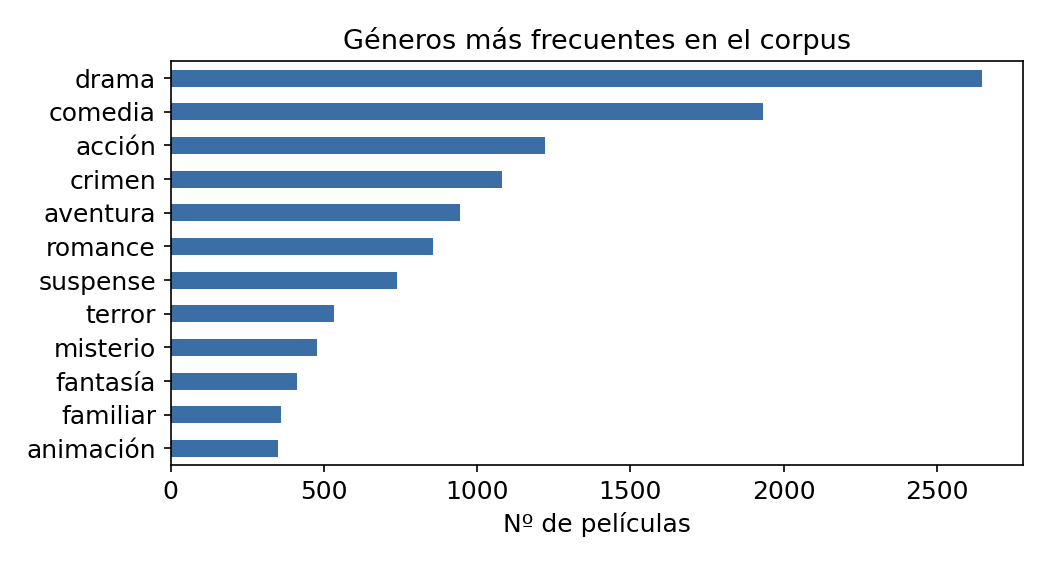
\includegraphics[width=\linewidth]{fig_generos.png}
    \end{column}
  \end{columns}
\end{frame}

\begin{frame}{Qué condiciona el corpus a nuestras decisiones}
  \begin{columns}
    \begin{column}{0.54\textwidth}
      \begin{itemize}
        \item \textbf{Idioma mixto:} las keywords mezclan español e inglés $\rightarrow$ el preprocesamiento usa stopwords de ambos.
        \item \textbf{Nombres duplicados} (61) $\rightarrow$ trabajamos con un índice interno, no con el título.
        \item \textbf{Historial incompleto:} de 64 películas vistas, 7 no están en el corpus.
        \item Lo importante: esas ausencias \textbf{no son aleatorias}, caen todas en los perfiles ambiguos.
      \end{itemize}
    \end{column}
    \begin{column}{0.46\textwidth}
      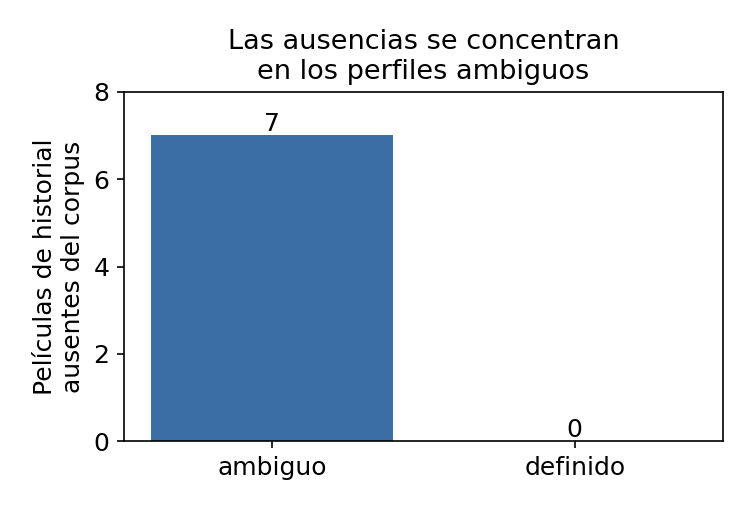
\includegraphics[width=\linewidth]{fig_ausencias.png}
    \end{column}
  \end{columns}
  \vspace{0.3em}
  \footnotesize Consecuencia: los usuarios más difíciles de modelar son, además, los que menos historial conservan.
\end{frame}

\begin{frame}{Por qué dos estrategias distintas}
  \begin{itemize}
    \item La pregunta de fondo: ¿cómo hacer que películas similares queden cerca en el espacio, y que ``similar'' signifique lo mismo para el sistema y para el usuario?
    \item Elegimos dos representaciones que entienden la similitud de maneras opuestas:
  \end{itemize}
  \vspace{0.5em}
  \centering
  \begin{tabular}{>{\raggedright}p{0.30\textwidth} p{0.30\textwidth} p{0.30\textwidth}}
    \toprule
     & \textbf{LDA (Estrategia 1)} & \textbf{LLM local (Estrategia 2)} \\
    \midrule
    Naturaleza & Tópicos latentes (probabilístico) & Razonamiento semántico \\
    Similitud & Compartir tópicos & Compartir sentido / intención \\
    Lectura & Transparente e interpretable & Caja negra con justificación \\
    \bottomrule
  \end{tabular}
\end{frame}

\section{Estrategia 1: Tópicos (LDA)}

\begin{frame}{Estrategia 1 --- modelado de tópicos con LDA}
  \begin{itemize}
    \item Sobre \texttt{sinopsis + keywords + género} entrenamos un \textbf{LDA} de 20 tópicos (\texttt{CountVectorizer} + \texttt{LatentDirichletAllocation}, como en la Unidad 3).
    \item Cada película queda descripta como una \textbf{distribución de tópicos} $\theta$ (una mezcla, no una etiqueta única).
    \item Qué esperamos que capture: los \emph{temas} del corpus (crimen, guerra, romance, ciencia ficción\dots) de forma interpretable.
    \item Ventaja sobre TF-IDF: no solo mide coincidencia de palabras, sino que agrupa vocabulario que aparece junto en un mismo tema.
  \end{itemize}
\end{frame}

\begin{frame}{Los tópicos que emergen}
  \centering
  \begin{tabular}{c l}
    \toprule
    \textbf{Tópico} & \textbf{Palabras más probables (interpretación)} \\
    \midrule
    T7  & crimen, policial, agente, asesinato, FBI \quad \textit{(policial)} \\
    T11 & guerra, bélico, mundial, Vietnam \quad \textit{(bélico)} \\
    T2  & terror, suspenso, misterio, asesino, horror \quad \textit{(terror/thriller)} \\
    T13 & ciencia ficción, alienígenas, futuro, viaje \quad \textit{(sci-fi)} \\
    T6  & relaciones, romance, familia, hijos \quad \textit{(drama familiar)} \\
    T10 & animación, aventura, fantasía, animal \quad \textit{(animación)} \\
    \bottomrule
  \end{tabular}
  \vspace{0.6em}
  \par\footnotesize Los tópicos son legibles: esto es lo que hace defendible e interpretable a la estrategia.
\end{frame}

\begin{frame}{Cómo representamos al usuario}
  \begin{itemize}
    \item El \textbf{historial} y la \textbf{query} aportan información distinta:
      \begin{itemize}
        \item historial = \emph{qué le gustó} (distribución promedio de tópicos de lo que vio);
        \item query = \emph{qué quiere ahora} (la proyectamos al modelo con \texttt{lda.transform}).
      \end{itemize}
    \item Perfil del usuario $= \alpha \cdot \text{tópicos(historial)} + (1-\alpha)\cdot \text{tópicos(query)}$.
    \item Recomendamos por \textbf{similitud coseno} en el espacio de tópicos, excluyendo lo ya visto.
    \item Si una película del historial no está en el corpus, se saltea (trabajamos con el \texttt{df} crudo).
  \end{itemize}
\end{frame}

\section{Resultados de la Estrategia 1}

\begin{frame}{Resultados LDA --- un acierto y un caso difícil}
  \begin{columns}
    \begin{column}{0.5\textwidth}
      \textbf{Rodrigo} (definido) \\
      \footnotesize\textit{``hechos reales sobre corrupción o poder político''}
      \begin{itemize}\footnotesize
        \item Tópicos del perfil: \textbf{T7 policial}, T0 biografía, \textbf{T11 bélico}.
        \item Recomienda: \textit{Canción triste de Hill Street}, \textit{Bajo el fuego} (bélico), \textit{The Staircase} (documental crimen).
        \item Captura el eje \emph{crimen/poder}, aunque pierde el matiz ``basado en hechos reales''.
      \end{itemize}
    \end{column}
    \begin{column}{0.5\textwidth}
      \textbf{Paula} (ambiguo) \\
      \footnotesize\textit{``no quiero pensar mucho, algo intermedio''}
      \begin{itemize}\footnotesize
        \item Tópicos del perfil: T17 romance/comedia, T5 documental --- señales que se contradicen.
        \item Recomienda: \textit{Antes de amanecer}, \textit{Philadelphia}, \textit{Tango para tres}: coherentes entre sí, pero la query casi no aporta dirección.
      \end{itemize}
    \end{column}
  \end{columns}
  \vspace{0.4em}
  \footnotesize La diferencia no está en el modelo sino en la \textbf{señal}: el perfil ambiguo no apunta a un lugar único del espacio.
\end{frame}

\begin{frame}{Evaluación de la Estrategia 1}
  \begin{columns}
    \begin{column}{0.56\textwidth}
      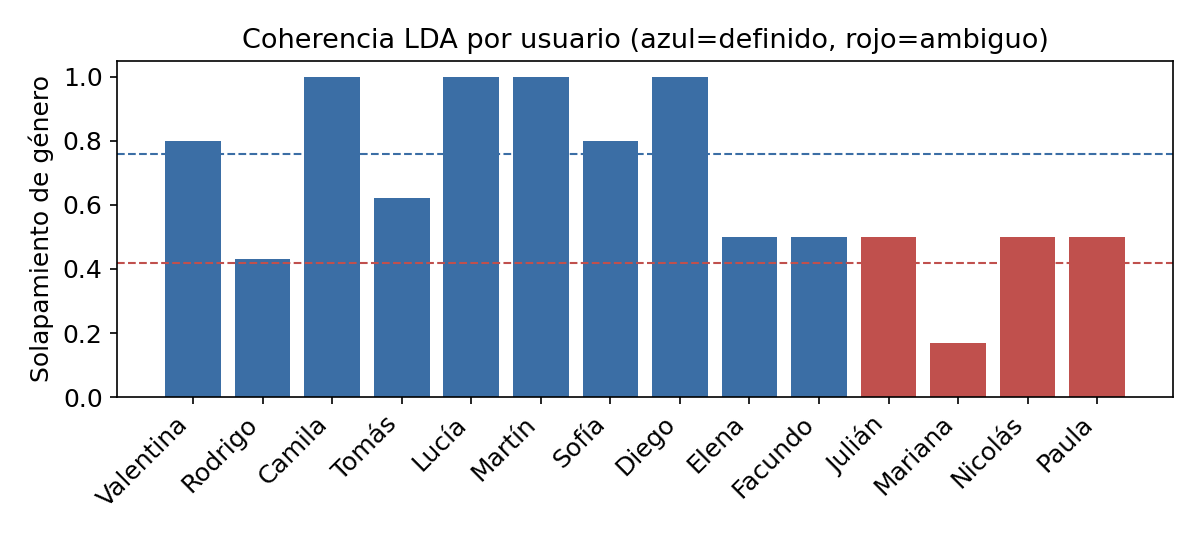
\includegraphics[width=\linewidth]{fig_eval_lda.png}
    \end{column}
    \begin{column}{0.44\textwidth}
      \begin{itemize}
        \item Sin \textit{ground truth}, usamos una proxy: solapamiento de género entre recomendaciones e historial.
        \item Promedio \textbf{definidos 0.76} vs \textbf{ambiguos 0.42}.
        \item El sistema se comporta como esperábamos: más coherente donde hay señal clara.
        \item La métrica \textbf{no es igualmente válida} para todos: en los ambiguos el propio historial es contradictorio.
      \end{itemize}
    \end{column}
  \end{columns}
\end{frame}

\section{Estrategia 2: LLM local}

\begin{frame}{Del límite de LDA a la Estrategia 2}
  \begin{itemize}
    \item LDA captura el \emph{tema} pero no la \emph{intención}: no entiende ``algo que te haga pensar sobre qué es real'' ni negaciones (``que no sea muy larga'').
    \item Estrategia 2 --- \textbf{LLM local con Ollama} (Unidad 5), en dos pasos (esquema RAG):
      \begin{enumerate}
        \item \textbf{Recuperación:} TF-IDF preselecciona un \textit{shortlist} de candidatos plausibles.
        \item \textbf{Reordenamiento:} el LLM lee historial + query + sinopsis y elige las 5 finales con un \textbf{motivo}.
      \end{enumerate}
    \item Restringir al shortlist evita que el modelo \emph{alucine} títulos fuera del corpus.
    \item Salida forzada a un \textbf{esquema Pydantic} (JSON parseable), como en la clase de Ollama.
  \end{itemize}
\end{frame}

\begin{frame}{Resultados de la Estrategia 2 (LLM)}
  \textbf{Rodrigo} (definido) --- \textit{``corrupción o poder político, basado en hechos reales''}
  \begin{itemize}\footnotesize
    \item \textit{Buenas noches y buena suerte}, \textit{El asesinato de Richard Nixon}, \textit{La verdad oculta}, \textit{El príncipe de la ciudad}, \textit{La noche cae sobre Manhattan}.
    \item Motivo (\textit{La verdad oculta}): ``basada en hechos reales; denuncia el encubrimiento de abusos por parte de la ONU''.
  \end{itemize}
  \textbf{Paula} (ambiguo) --- \textit{``algo intermedio, ni vacío ni pesado''}
  \begin{itemize}\footnotesize
    \item \textit{Beautiful Girls}, \textit{Intimidad}, \textit{Gintama}, \textit{El último americano virgen}, \textit{2046}.
    \item Motivo (\textit{Beautiful Girls}): ``permite reflexionar sobre la vida sin sentirse abrumado''.
  \end{itemize}
  \vspace{0.3em}
  \footnotesize En Rodrigo el LLM capta el matiz \textbf{``basado en hechos reales''} que LDA no distinguía (4 de 5 son sobre corrupción real); en Paula verbaliza el ``intermedio'' que pedía, pero las elecciones quedan heterogéneas: cuando no hay señal, el LLM la \emph{explica} mejor, no la \emph{inventa}.
\end{frame}

\section{Comparación y cierre}

\begin{frame}{LDA frente a LLM}
  \centering
  \begin{tabular}{p{0.26\textwidth} p{0.33\textwidth} p{0.33\textwidth}}
    \toprule
    & \textbf{LDA (tópicos)} & \textbf{LLM local} \\
    \midrule
    Qué compara & Tópicos compartidos & Significado / intención \\
    Matices y negación & No los capta & Los interpreta \\
    Interpretabilidad & Alta (tópicos legibles) & Baja, pero da un motivo \\
    Reproducibilidad & Total (determinista) & No determinista \\
    Costo & Milisegundos & Segundos por usuario \\
    Riesgo & Tópicos difusos & Alucinar fuera de lista \\
    \bottomrule
  \end{tabular}
  \vspace{0.5em}
  \par\footnotesize No compiten: LDA da estructura interpretable; el LLM aporta comprensión de la query. Se complementan.
\end{frame}

\begin{frame}{Límites del enfoque basado en contenido}
  \begin{itemize}
    \item Hay un techo que \textbf{más datos del mismo tipo no resuelven}:
      \begin{itemize}
        \item sin señal de otros usuarios, no hay descubrimiento por gustos parecidos (filtrado colaborativo);
        \item una query vaga es vaga para cualquier representación;
        \item evaluar sin \textit{ground truth} obliga a proxies imperfectas.
      \end{itemize}
    \item Lo que sí mejoraría: keywords más completas, sinopsis más largas, o señales de feedback del usuario.
  \end{itemize}
\end{frame}

\begin{frame}{Conclusión y recomendación}
  \begin{itemize}
    \item Ambas estrategias \textbf{funcionan bien en perfiles definidos} y se degradan en los ambiguos: el límite es la señal, no el método.
    \item \textbf{Recomendación:} usar el \textbf{LLM} como recomendador principal por su lectura de la intención, con \textbf{LDA} como capa interpretable para explicar y auditar las recomendaciones.
    \item Para perfiles con poca señal, el sistema debería \textbf{pedir más información} antes que arriesgar una recomendación pobre.
  \end{itemize}
  \vspace{0.6em}
  \centering \footnotesize ¿Preguntas?
\end{frame}

\end{document}
